%
% ─── CAPITULO 8: VISUALIZACION DE FRACTALES 3D ──────────────────────────────────
%

En el capítulo \ref{chap:fractales-2D} introdujimos técnicas y código necesario para poder visualizar conjuntos de Julia y conjuntos de Mandelbrot 2-dimensionales en un canvas utilizando WebGL, todo ello apoyado en la teoría explicada en el capítulo \ref{chap:Julia-Mandelbrot}. Sin embargo, el objetivo de éste y de los tres capítulos anteriores es aplicar técnicas avanzadas de renderizado para poder visualizar fractales en tres dimensiones. Recordamos que explicamos en la introducción del capítulo \ref{chap:ray-tracing} que la mejor forma de renderizar fractales 3D es utilizando la técnica de `Ray Tracing', que en dicho capítulo explicamos con detalle. A pesar de ello y de conseguir escenas con varios objetos, materiales y movimientos de cámara no visualizamos nada lejanamente parecido a un fractal. Será en este capítulo en el que aprovecharemos toda la infraestructura y todo el código implementado hasta el momento en el `ray-tracer' del capítulo \ref{chap:ray-tracing} para graficar fractales tridimensionales.

Para ello, antes aún debemos asentar una serie de conceptos que son los que nos ayudarán a cumplir nuestro objetivo: el algoritmo \textit{Ray-Marching} y las conocidas como \textit{Signed Distance Functions} (SDFs). Con estos dos elementos combinados conseguiremos ver hermosas figuras fractales.

\section{El algoritmo Ray-Marching}
\label{section:ray-arching}

Hasta ahora siempre hemos calculado las intersecciones rayo-esfera de manera totalmente analítica, ya que es muy sencillo describir una esfera o un plano mediante una ecuación y solucionar esta ecuación en $t$, como vimos en las secciones \ref{subsection:esfera} y \ref{subsection:plano}. Sin embargo, no es tan sencillo encontrar ecuaciones que describan la superficie de los fractales. Es por esto que necesitamos otra manera de encontrar las intersecciones rayo-superficie. Aunque no tengamos una forma de calcular analíticamente la intersección, si contamos con funciones que nos estiman, fijado un punto, a qué distancia se halla este punto del fractal mediante una cota, las conocidas como SDFs (sección \ref{section:SDFs}). De igual manera, si fijamos un punto $p\in\R^3$, podemos calcular a qué distancia se encuentra dicho punto de una esfera o de un plano. 

El algoritmo \textit{Ray-Marching}, también conocido como \textit{Sphere-Tracing} es una técnica utilizada en Ray-Tracing y que se basa en estimar la distancia a la que se encuentra un punto de cada una de las superficies que componen la escena y avanzar en el rayo una distancia correspondiente a la mínima de estas distancias, pues se tiene la certeza de que al menos en una esfera de radio dicha distancia no hay ninguna intersección con ningún otro cuerpo. Una vez se ha avanzado en el rayo se repite esta operación y así sucesivamente hasta que la estimación de la distancia es lo suficientemente pequeña como para considerar que el punto interseca con la superficie. Los fundamentos matemáticos de este método y las propiedades que deben cumplir las funciones estimadoras se pueden encontrar en \cite{Hart-1995}. 

Pongamos un ejemplo. Supongamos que tenemos una escena con una esfera tangente al plano horizontal $y=0$, un rayo $R$ fijo y queremos aplicar Ray-Marching para encontrar la intersección.

\begin{figure} [ht]
    \centering
    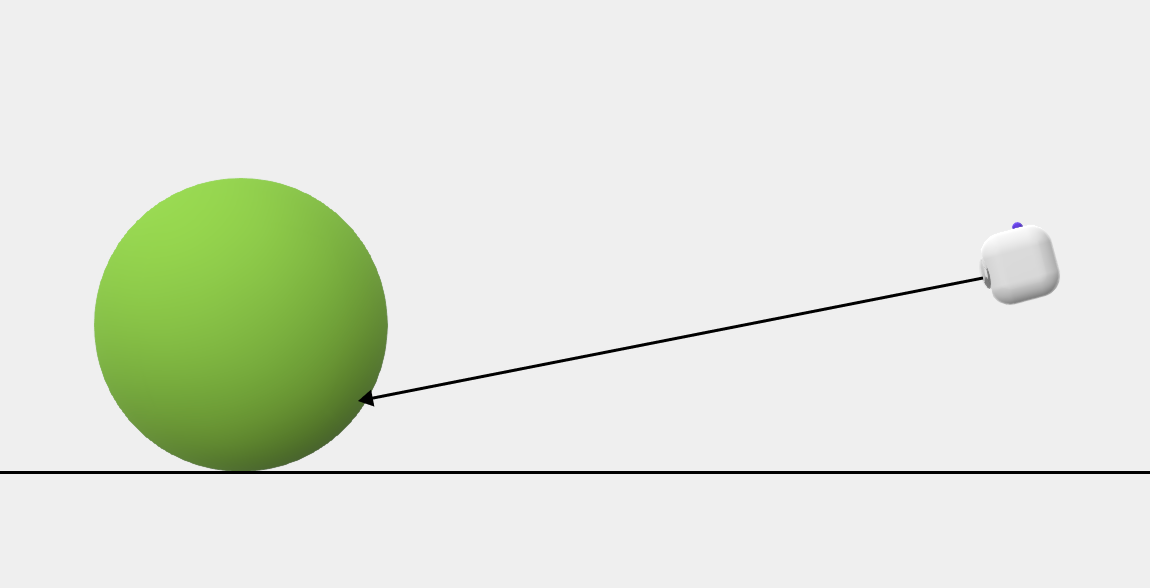
\includegraphics[scale = 0.2]{img/C8/situacion-inicial.png}
    \caption{Situación a la que aplicar Ray-Marching}
    \label{fig:RM-inicial}
\end{figure}

La distancia de un punto $p$ a una esfera $S$ de centro $c$ y radio $r$ es 
\begin{equation}
    \label{eq:distancia-punto-esfera}
    d(p,S) = \|p-c\| - r 
\end{equation}

y la distancia de un punto al plano $y=0$ es simplemente su componente $y$. Por tanto, partiendo del origen, calculamos la distancia a la esfera y la distancia al plano, vemos que es menor la distancia al plano, por lo que avanzamos en el rayo una distancia igual a la distancia que había al plano (imagen \ref{fig:iteraciones-RM} (a)). Seguidamente repetimos la operación: volvemos a calcular la distancia a la esfera y al plano. De nuevo es menor la distancia al plano, por lo que avanzamos en el rayo la misma distancia que había en el plano (imagen \ref{fig:iteraciones-RM} (b)).

\begin{figure}[ht]
    \centering
    \begin{tabular}{ccc}
      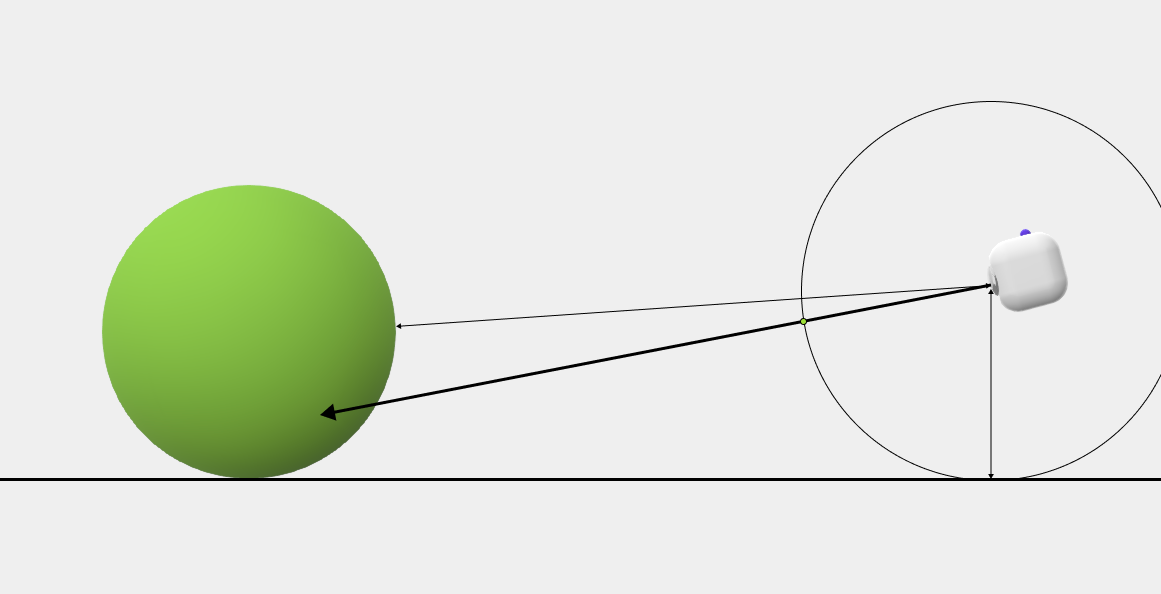
\includegraphics[scale=0.17]{img/C8/ray-marching-1.png} &     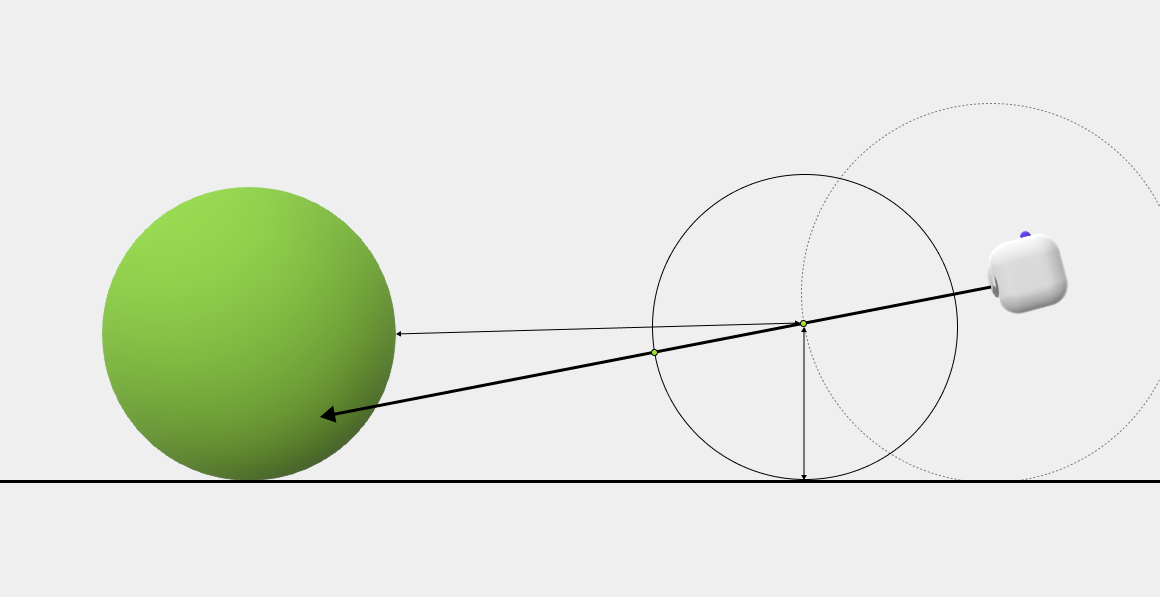
\includegraphics[scale=0.17]{img/C8/ray-marching-2.png} \\
    (a) Primera iteración & (b) Segunda iteración \\[6pt]
    \end{tabular}
    \caption{Dos primeras iteraciones de Ray Marching}
    \label{fig:iteraciones-RM}
\end{figure}

Si repetimos este proceso indefinidamente, llegará el momento en el que la distancia a la esfera será tan pequeña que consideraremos que el punto está en la esfera y habremos encontrado la intersección (imagen \ref{fig:finales} (a)). En caso de que no exista ninguna intersección, el algoritmo seguirá avanzando en el rayo, pero al no intersecar con ninguna superficie se avanzará indefinidamente (imagen \ref{fig:finales} (b)), por lo que hay que fijar una distancia máxima recorrida o un número máximo de iteraciones como parámetro del algoritmo.

\begin{figure}[ht]
    \centering
    \begin{tabular}{ccc}
      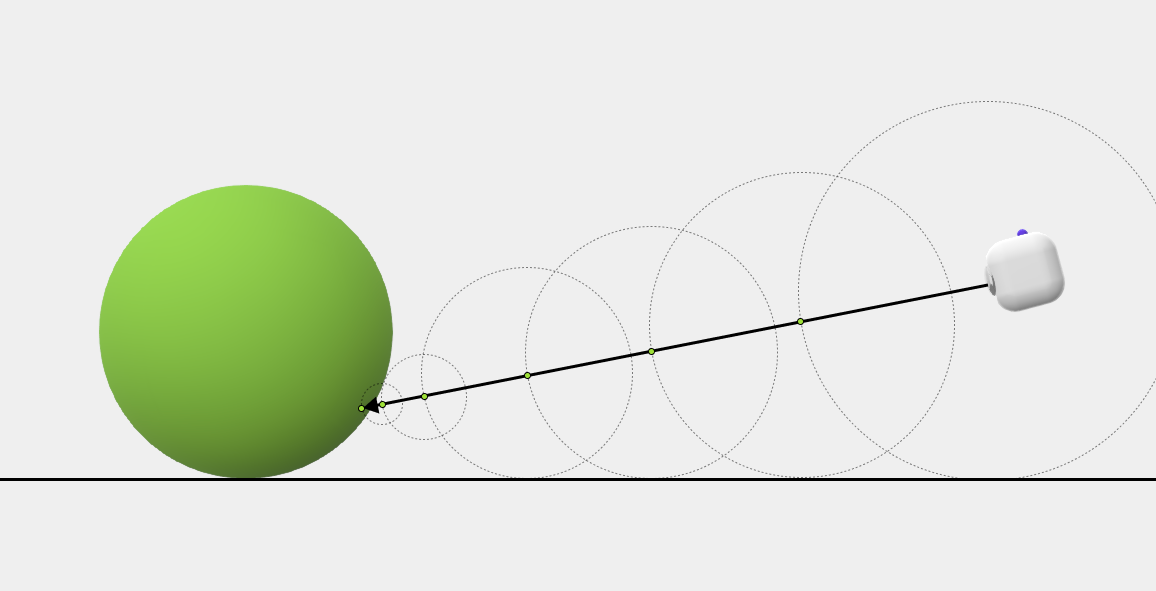
\includegraphics[scale=0.2]{img/C8/ray-marching-final.png} &     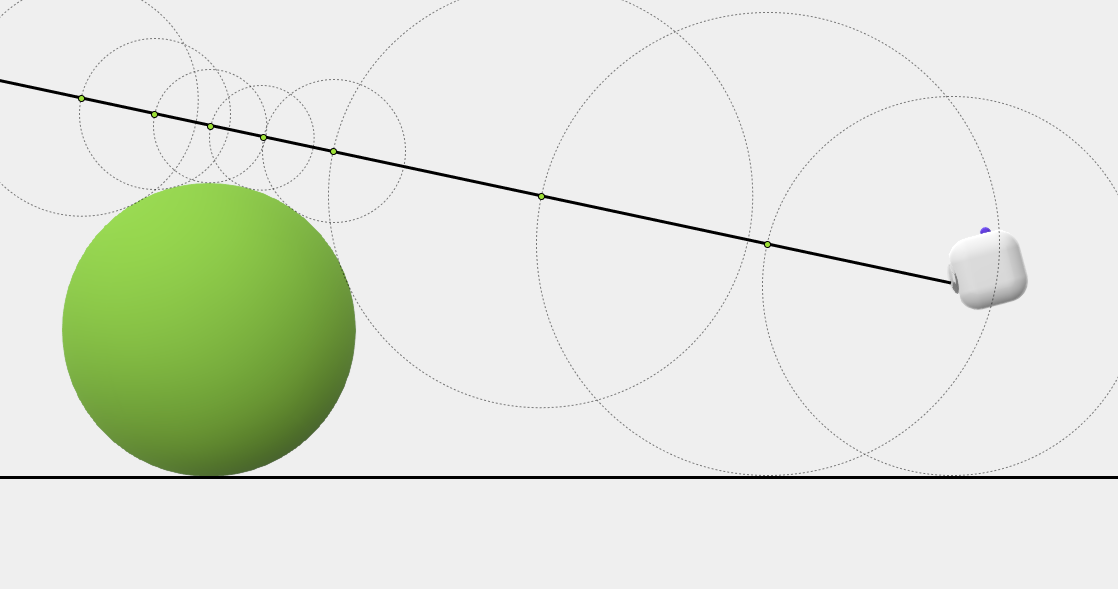
\includegraphics[scale=0.2]{img/C8/ray-marching-miss.png} \\
    (a) Encuentra intersección & (b) El rayo se pierde \\[6pt]
    \end{tabular}
    \caption{Posibles estados finales del algoritmo Ray-Marching}
    \label{fig:finales}
\end{figure}

Por tanto, el algoritmo, si consideramos un conjunto de $objetos$, un rato $R(t)=p_0 + \vec v t$ y un número máximo de avances en el rayo antes de decidir que no existe intersección $MAX\_STEPS$, se describiría como indica el algoritmo \ref{alg:Ray-Marching}.

\begin{algorithm}[H]
\caption{Ray-Marching} \label{alg:Ray-Marching}
%\KwData{Objects: Array de objetos, $\epsilon$: Distancia por debajo de la cual se considera intersección, R: Rayo $R(t)=p_0+\vec v t$}
\begin{algorithmic}
\State $p\gets lookfrom$
\State $steps \gets 0$

\While{$steps < MAX\_STEPS$} \Comment{También se puede fijar una distancia máxima}
    \State $min\_dist \gets MAX\_DIST$
    \State $i\gets 0$

    
    \While{$i < num\_objects$}\Comment{Cálculo de la mínima distancia}
        \State $dist \gets distancia(p, objects[i])$
        \If{$dist < min\_dist$}
            \State $min\_dist \gets dist$
            \State $index\gets i$
        \EndIf
        \State $i++$
    \EndWhile
    \If{$min\_dist < \varepsilon$}
        \State \textbf{Hay intersección} con $objects[index]$
    \Else
        \State $p\gets p + \vec v \cdot min\_dist$ \Comment{Avanzamos en el rayo}
    \EndIf
    \State $steps++$
\EndWhile
\State \textbf{No existe intersección}
\end{algorithmic}
\end{algorithm}

\begin{observacion}
\label{observacion:vector-normalizado}
    Cabe destacar un importante detalle, y es que a partir de este momento es indispensable que en la creación del rayo el vector dirección esté normalizado, pues si queremos avanzar $min\_dist$ unidades en la dirección $\vec v$ y $|v| \not= 1$ se avanzaría una distancia distinta y el algoritmo no funcionaría correctamente.
\end{observacion}

\subsection{Implementación de Ray-Marching en GLSL}

Veámos ahora cómo podemos llevarnos todos estos nuevos conocimientos a la GPU con GLSL. El objetivo ahora es modificar el fragment shader eliminando la dependencia de \verb|Hit_Sphere| y de \verb|Hit_Plane| para utilizar Ray-Marching para calcular las intersecciones. Realmente el resultado de estas modificaciones debería ser el mismo que en el final del capítulo anterior, pero ahora calcularemos las intersecciones de forma distinta. 

Lo primero que necesitaremos es una función que calcule la distancia de un punto a una esfera $S$. Esto es tan sencillo como implementar una función que calcule la fórmula \ref{eq:distancia-punto-esfera}.

\begin{lstlisting}
// Dada una esfera S y un punto p, calcula la distancia
// del punto a la superficie de la esfera
float get_dist_sphere(vec3 p, Sphere S){
    return length(S.center - p) - S.radius;
}
\end{lstlisting}

Por parte del plano, podríamos aprovechar que nuestro plano es el $y=-2$ y simplemente devolver la componente $y$ del punto más dos. Sin embargo, no cuesta tanto calcular la distancia de un punto a un plano arbitrario $Ax+By+Cz = D$, siendo $\vec N=(A,B,C)$ el vector normal al plano. El punto perteneciente a un plano más cercano a otro punto $p$ dado es aquel que interseca con la recta cuyo vector director es el normal al plano y que pasa por $p$. Es decir, el punto de la recta $S(t)=p+\vec Nt$ que satisface la ecuación $(A,B,C)\cdot (x,y,z) = D$. Veámos para qué $t$ se satisfacen las ecuaciones.
\begin{equation}
    \begin{split}
        \vec N\cdot S(t) &= D \\
        \vec N\cdot (p+\vec N t) &= D \\
        t &= \dfrac{D-\vec N \cdot p}{|\vec N|^2}
    \end{split}
\end{equation}
Por tanto la distancia entre punto y plano es la longitud del vector que une a $p$ con $S(t)$, siendo este $t$ el recién calculado. El código entonces sería:
\begin{lstlisting}
// Dado un plano P y un punto p, calcula la distancia del 
// punto p a la superficie del plano.
float get_dist_plane (vec3 p, Plane P) {
    float t_interseccion = (P.D - dot(P.normal,p))/dot(P.normal, P.normal);
    vec3 closest_point = p + t_interseccion * P.normal;
    return length(p-closest_point);
}
\end{lstlisting}

Seguidamente necesitamos fijar dos constantes: el número máximo de iteraciones que se darán en el algoritmo y $\varepsilon$, la distancia mínima por debajo de la misma se considera que un punto pertenece a la superficie. La primera de ellas la podemos tomar como una macro, al igual que hicimos con el tamaño de los arrays, pero la segunda interesa que sea parametrizable, para así poder observar los niveles de detalle y qué variaciones experimenta la escena al modificar este valor. Por ello, usamos una variable \verb|uniform| a la que pasaremos valor vía JavaScript.

\begin{lstlisting}
    uniform float u_epsilon;
    // ... 
    #define MAX_STEPS 1000
\end{lstlisting}

Y ya tenemos todo preparado para implementar el Ray-Marching. La función que dado un rayo calcula posibles intersecciones con los cuerpos y asigna un color en función es \verb|ray_color|, por lo que lo más natural es editar el código de esta función. En lugar de llamar a \verb|hit_sphere_list| y \verb|hit_plane| como hicimos en la sección \ref{subsection:plano} aplicaremos Ray-Marching. Como GLSL no nos permite mantener un array heterogéneo en el que almacenar todos los objetos independientemente de su tipo, tenemos que hacerlo de forma secuencial. Y como tampoco permite acceder a elementos de un array a partir de índices no constantes, utilizaremos una variable donde almacenar la esfera más cercana, para recuperarla en caso de intersección, véase el código.

\begin{lstlisting}
vec4 ray_color(Ray r, Sphere S[ARRAY_TAM], int num_spheres, 
    Plane ground,
    Directional_light lights[ARRAY_TAM], int num_lights) {
    
    Hit_record hr; hr.hit = false;  // Hit_record structure
    float dist = MAX_DIST;          // Distancia a cada objeto 
    vec3 p = r.orig;                // Punto del rayo
    float closest_dist = MAX_DIST;  // Menor distancia
    float current_t = 0.0;          // p=orig+current_t*dir
    vec4 tmp_color;                 // Color temporal
    Sphere S_hit;                   // Esfera mas cercana
    
    int object_index;   // 0,...,num_spheres-1: esferas,
                        // num_spherees: plano
    // Ray Marching
    for(int i = 0; i < MAX_STEPS; i++) {
        // Calculamos el objeto mas cercano
        closest_dist = MAX_DIST;

        // Distancia a las esferas
        for(int i = 0; i < ARRAY_TAM; i++) {
            if(i == num_spheres) break;
            dist = get_dist_sphere(p, S[i]);
            if(dist < closest_dist) {
                closest_dist = dist;
                object_index = i;
                S_hit = S[i];
            }
        }

        // Distancia al suelo
        dist = get_dist_plane(p, ground);
        if(dist < closest_dist) {
            closest_dist = dist;
            object_index = num_spheres;
        }
    
        // closest_dist almacena la menor de las distancias
        // y object_index el indice del objeto mas cercano
        if(closest_dist < u_epsilon){   // Hay interseccion

            hr.hit = true;
            hr.t = current_t;
            hr.p = ray_at(r, hr.t);

            if(object_index == num_spheres){ // Suelo
                // Codigo de interseccion con el suelo ...
            }

            else {      // Una de las esferas
                // Codigo de interseccion con S_hit
            }
        }

        // Si no hay interseccion, avanzamos en el rayo
        current_t += closest_dist;
        p = ray_at(r, current_t);

        // Si estamos muy lejos acabamos el bucle
        if(current_t >= MAX_DIST) break;
    }
    // No hay interseccion
    // Background code ...       
}
\end{lstlisting}

Fíjese que concuerda con la estructura que describe el algoritmo \ref{alg:Ray-Marching}. Hecha esta modificación, el resultado fijando ciertos parámetros dinámicamente es el mostrado en la imagen \ref{fig:esferas-RM}. Tal y como adelantamos, el resultado es igual que cuando calculábamos las intersecciones exactas, ya que realmente lo único que cambia es la forma de calcular las intersecciones, nada estrictamente visual.

\begin{figure} [ht]
    \centering
    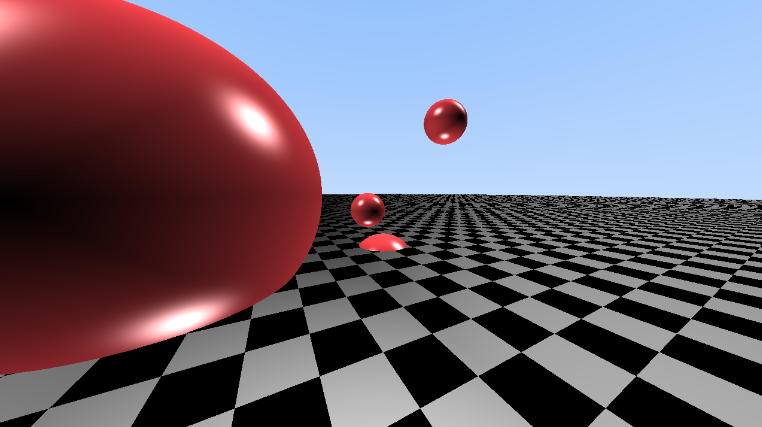
\includegraphics[scale = 0.37]{img/C8/esferas-ray-marching.png}
    \caption{Escena tras implementar Ray-Marching}
    \label{fig:esferas-RM}
\end{figure}

Recordamos e insistimos en que el vector director del rayo \verb|r.dir| debe ser un vector normalizado, es decir, unitario. De otro modo los avances en el rayo no estarán controlados, obsérvese en la imagen \ref{fig:vectores-no-normalizados} los resultados obtenidos al no normalizar el vector director al crear el rayo.

\begin{figure} [ht]
    \centering
    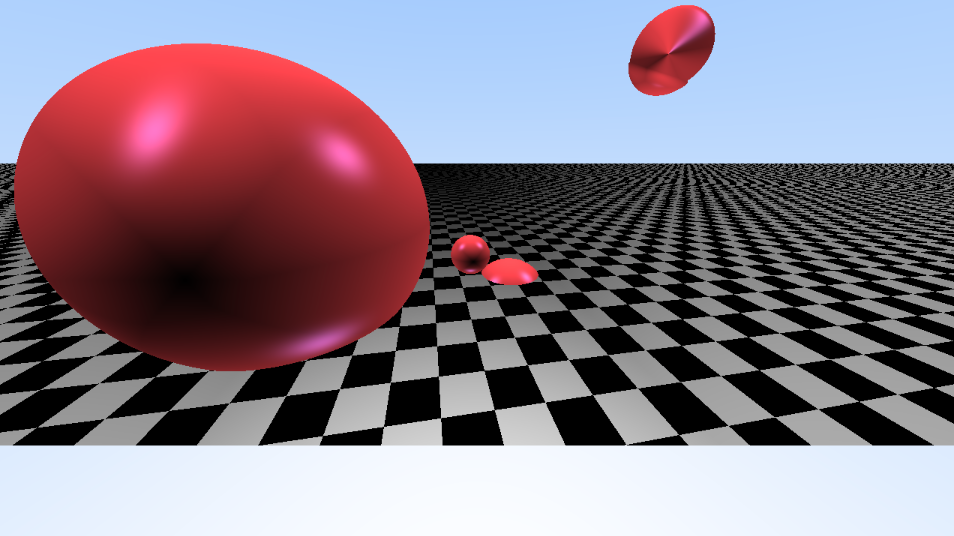
\includegraphics[scale = 0.3]{img/C8/vectores-no-normalizados.png}
    \caption{Escena utilizando vectores no unitarios en los rayos}
    \label{fig:vectores-no-normalizados}
\end{figure}

\subsection{Comentarios sobre Ray-Marching}

Una vez hemos introducido e implementado el algoritmo Ray-Marching, el lector es posible que piense que es una forma menos exacta y además menos eficiente que calcular analíticamente las intersecciones con los cuerpos. Es cierto que en casos como el de esferas o planos cuyas ecuaciones implícitas y sus intersecciones con rayos están muy bien definidos y son sencillas de calcular aplicar ray-marching ralentiza el procesado. Sin embargo muchas superficies, como es el caso de los fractales, no cuentan con una ecuación implícita que la defina. Otras sí cuentan con ecuaciones implícitas pero estas son muy difíciles de resolver. En este último caso se pueden aplicar métodos numéricos para aproximar las soluciones, que son métodos precisamente iterativos. 

Sin embargo, ray-marching sólo necesita, para cada cuerpo, una función que aproxime suficientemente bien la distancia a un conjunto. A partir de un rayo y dichas funciones se puede aplicar ray-marching, de forma que se converge finalmente al punto de intersección. Por contra, si buscamos intersecciones analíticas hay que resolver ecuaciones, en ocasiones para acabar aproximando las soluciones, y retener la más pequeña.

Un aspecto a destacar de ray-marching es la dependencia de sus parámetros. Es importante fijar un valor $\varepsilon$ adecuado, ya que si es demasiado grande puede brindarnos resultados muy pobres. En la imagen \ref{fig:esferas-RM} se ha utilizado $\varepsilon=0.001$ y nos da un resultado muy bueno, pero obsérvese en la imagen \ref{fig:epsilon-grande} qué ocurre si se fija $\varepsilon=0.1$. Los límites de los cuadrados del suelo se distorsionan y las apariencias de las esferas también se ven muy resentidas. Sin embargo es cierto que a mayor valor de $\varepsilon$ menos iteraciones y por tanto más velocidad, pero los resultados son peores. Es por tanto necesario utilizar valores de $\varepsilon$ adecuados a la situación, siendo suficientemente pequeños como para obtener un buen resultado pero suficientemente grandes como para que sea computacionalmente viable.

\begin{figure} [ht]
    \centering
    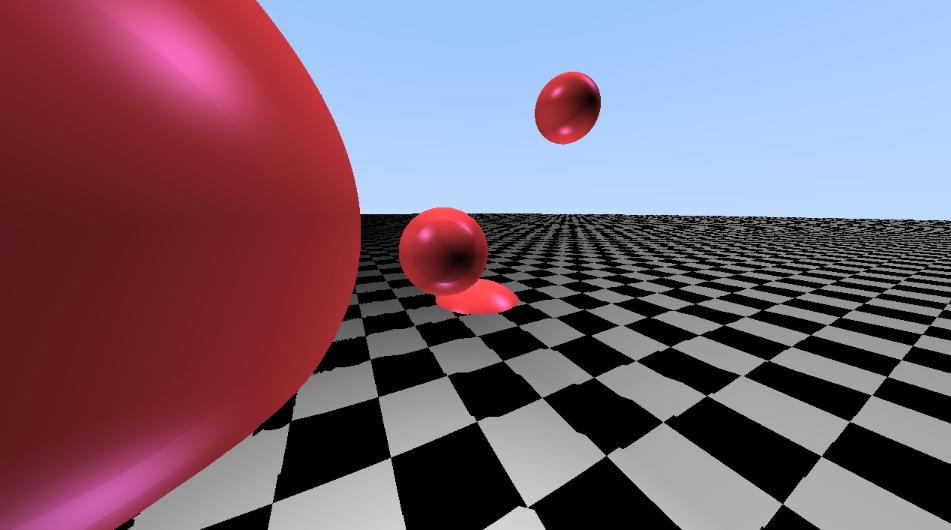
\includegraphics[scale = 0.3]{img/C8/epsilon-grande.png}
    \caption{Escena renderizada utilizando $\varepsilon=0.1$}
    \label{fig:epsilon-grande}
\end{figure}

Una reflexión similar se puede aplicar al parámetro que define el número máximo de iteraciones (\verb|MAX_STEPS|). Pensemos en un rayo que pasa muy cerca de un objeto pero no llega a intersecarlo, sino que finalmente interseca al suelo. Durante las iteraciones que el rayo pase cerca del objeto quizá avance muy lentamente durante varias iteraciones, pues la distancia mínima es la distancia a dicho objeto que es pequeña. Este hecho puede provocar que se alcance el número máximo de iteraciones, considerando así que el rayo no golpea ningún objeto y asignándole el color de fondo cuando realmente con algunas iteraciones más podría alcanzarse la intersección con el suelo. Este hecho se puede observar en la imagen \ref{fig:pocas-iteraciones}, donde se ha utilizado \verb|MAX_STEPS=100|. Fíjese en las fronteras entre el horizonte y las esferas, o en los bordes de las esferas.

\begin{figure} [ht]
    \centering
    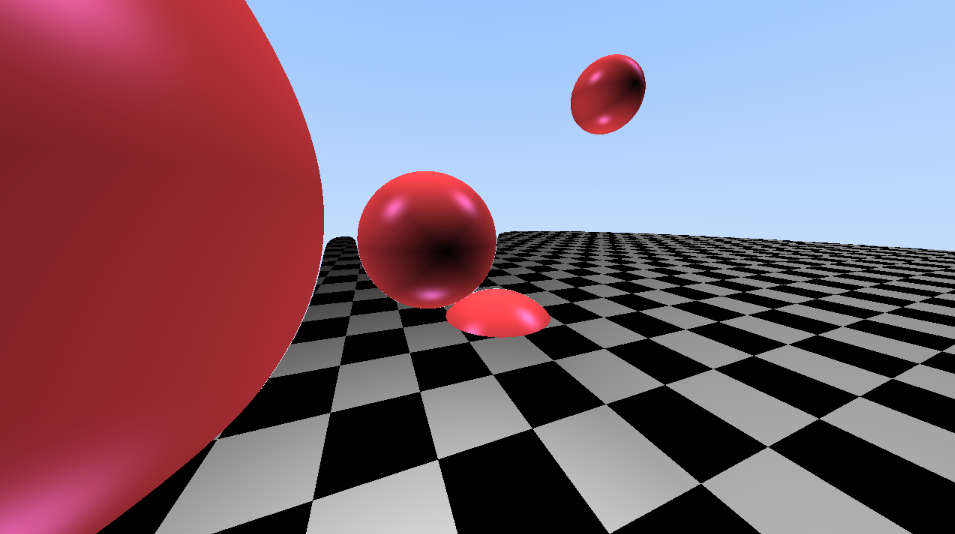
\includegraphics[scale = 0.3]{img/C8/pocas-iteraciones.png}
    \caption{Escena renderizada utilizando MAX\_STEPS=100}
    \label{fig:pocas-iteraciones}
\end{figure}

De igual forma, menos iteraciones implica más rapidez, pero peores resultados, por lo que es necesario fijar un valor correcto.

\section{Signed Distance Functions (SDFs)}
\label{section:SDFs}

Durante toda la sección anterior hemos hablado de que para aplicar ray-marching es necesario que cada objeto que componga la escena cuente con una función que estime la distancia de un punto cualquiera de $\R^3$ a su superficie. En esta sección introduciremos el concepto de SDF y explicaremos cómo obtener esas funciones para fractales 3D.

Primero explicaremos brevemente el fundamento matemático. Sea $f:\R^n\longrightarrow\R$ una función continua que define implícitamente el conjunto 
$$
A = \{x\in\R^n: f(x)\leq 0\}.
$$
Por continuidad, $f(x)=0\ \ \forall x\in\partial A$. Decimos que la frontera $\partial A$ define la \textit{superficie implícita} de $f$. De hecho, $f$ es negativa en el interior de $A$ ($f(x)<0 \ \ \forall x\in\mathring A$), por lo que podemos decir que dicha superficie implícita $\partial A$ coincide precisamente con el conjunto $f^{-1}(0)$. A partir de una función real y continua podemos entonces definir una superficie en $\R^n$.

\begin{definicion}[SDF]
    Una función continua $f:\R^3\longrightarrow\R$ se conoce como una \textbf{`Signed Distance Bound'} (distancia a la frontera con signo) de su superficie implícita $f^{-1}(0)$ si, y solo si
    \begin{equation}
        \label{eq:SDB}
        |f(x)|\leq d(x,f^{-1}(0)) \ \ \forall x\in\R^3
    \end{equation}
    
    Si se tiene la igualdad en (\ref{eq:SDB}), entonces $f$ es una \textbf{`Signed Distance Function'} (función distancia con signo).
\end{definicion}

Como ya hemos visto en la sección anterior, algunas primitivas, como las esferas, pueden ser fácilmente definidas por su SDF. Recordamos que la SDF de una esfera es $f(x)=|x-c|-r$ siendo $c\in\R^3$ su centro y $r\in\R$ su radio. Entonces un punto exterior a la esfera tendrá un valor de la SDF positivo, uno interior tendrá un valor negativo y únicamente se anulará en el caso de que el punto pertenezca a la superficie de la esfera. En \cite[Table 1]{Hart-1995} podemos encontrar una lista de primitivas con referencias a sus correspondientes SDFs.